% Graphic for TeX using PGF
% Title: /media/danilo/E472BA7972BA5052/Danilo/Documenti/Università/LatexTesiMagistrale/images/nonmanifold.dia
% Creator: Dia v0.97.3
% CreationDate: Fri Jan 29 16:46:21 2016
% For: danilo
% \usepackage{tikz}
% The following commands are not supported in PSTricks at present
% We define them conditionally, so when they are implemented,
% this pgf file will use them.
\ifx\du\undefined
  \newlength{\du}
\fi
\setlength{\du}{15\unitlength}
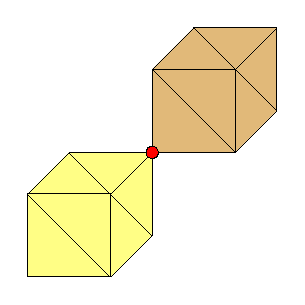
\begin{tikzpicture}
\pgftransformxscale{1.000000}
\pgftransformyscale{-1.000000}
\definecolor{dialinecolor}{rgb}{0.000000, 0.000000, 0.000000}
\pgfsetstrokecolor{dialinecolor}
\definecolor{dialinecolor}{rgb}{1.000000, 1.000000, 1.000000}
\pgfsetfillcolor{dialinecolor}
\pgfsetlinewidth{0.000000\du}
\pgfsetdash{}{0pt}
\pgfsetdash{}{0pt}
\pgfsetmiterjoin
\pgfsetbuttcap
\definecolor{dialinecolor}{rgb}{1.000000, 0.996078, 0.521569}
\pgfsetfillcolor{dialinecolor}
\fill (16.000000\du,15.000000\du)--(18.000000\du,15.000000\du)--(16.000000\du,13.000000\du)--cycle;
\definecolor{dialinecolor}{rgb}{0.000000, 0.000000, 0.000000}
\pgfsetstrokecolor{dialinecolor}
\draw (16.000000\du,15.000000\du)--(18.000000\du,15.000000\du)--(16.000000\du,13.000000\du)--cycle;
\pgfsetlinewidth{0.000000\du}
\pgfsetdash{}{0pt}
\pgfsetdash{}{0pt}
\pgfsetmiterjoin
\pgfsetbuttcap
\definecolor{dialinecolor}{rgb}{1.000000, 0.996078, 0.521569}
\pgfsetfillcolor{dialinecolor}
\fill (16.000000\du,13.000000\du)--(18.000000\du,15.000000\du)--(18.000000\du,13.000000\du)--cycle;
\definecolor{dialinecolor}{rgb}{0.000000, 0.000000, 0.000000}
\pgfsetstrokecolor{dialinecolor}
\draw (16.000000\du,13.000000\du)--(18.000000\du,15.000000\du)--(18.000000\du,13.000000\du)--cycle;
\pgfsetlinewidth{0.000000\du}
\pgfsetdash{}{0pt}
\pgfsetdash{}{0pt}
\pgfsetmiterjoin
\pgfsetbuttcap
\definecolor{dialinecolor}{rgb}{1.000000, 0.996078, 0.521569}
\pgfsetfillcolor{dialinecolor}
\fill (16.000000\du,13.000000\du)--(18.000000\du,13.000000\du)--(17.000000\du,12.000000\du)--cycle;
\definecolor{dialinecolor}{rgb}{0.000000, 0.000000, 0.000000}
\pgfsetstrokecolor{dialinecolor}
\draw (16.000000\du,13.000000\du)--(18.000000\du,13.000000\du)--(17.000000\du,12.000000\du)--cycle;
\pgfsetlinewidth{0.000000\du}
\pgfsetdash{}{0pt}
\pgfsetdash{}{0pt}
\pgfsetmiterjoin
\pgfsetbuttcap
\definecolor{dialinecolor}{rgb}{1.000000, 0.996078, 0.521569}
\pgfsetfillcolor{dialinecolor}
\fill (17.000000\du,12.000000\du)--(18.000000\du,13.000000\du)--(19.000000\du,12.000000\du)--cycle;
\definecolor{dialinecolor}{rgb}{0.000000, 0.000000, 0.000000}
\pgfsetstrokecolor{dialinecolor}
\draw (17.000000\du,12.000000\du)--(18.000000\du,13.000000\du)--(19.000000\du,12.000000\du)--cycle;
\pgfsetlinewidth{0.000000\du}
\pgfsetdash{}{0pt}
\pgfsetdash{}{0pt}
\pgfsetmiterjoin
\pgfsetbuttcap
\definecolor{dialinecolor}{rgb}{1.000000, 0.996078, 0.521569}
\pgfsetfillcolor{dialinecolor}
\fill (18.000000\du,15.000000\du)--(19.000000\du,14.000000\du)--(18.000000\du,13.000000\du)--cycle;
\definecolor{dialinecolor}{rgb}{0.000000, 0.000000, 0.000000}
\pgfsetstrokecolor{dialinecolor}
\draw (18.000000\du,15.000000\du)--(19.000000\du,14.000000\du)--(18.000000\du,13.000000\du)--cycle;
\pgfsetlinewidth{0.000000\du}
\pgfsetdash{}{0pt}
\pgfsetdash{}{0pt}
\pgfsetmiterjoin
\pgfsetbuttcap
\definecolor{dialinecolor}{rgb}{1.000000, 0.996078, 0.521569}
\pgfsetfillcolor{dialinecolor}
\fill (18.000000\du,13.000000\du)--(19.000000\du,14.000000\du)--(19.000000\du,12.000000\du)--cycle;
\definecolor{dialinecolor}{rgb}{0.000000, 0.000000, 0.000000}
\pgfsetstrokecolor{dialinecolor}
\draw (18.000000\du,13.000000\du)--(19.000000\du,14.000000\du)--(19.000000\du,12.000000\du)--cycle;
\pgfsetlinewidth{0.000000\du}
\pgfsetdash{}{0pt}
\pgfsetdash{}{0pt}
\pgfsetmiterjoin
\pgfsetbuttcap
\definecolor{dialinecolor}{rgb}{0.882353, 0.725490, 0.474510}
\pgfsetfillcolor{dialinecolor}
\fill (19.000000\du,12.000000\du)--(21.000000\du,12.000000\du)--(19.000000\du,10.000000\du)--cycle;
\definecolor{dialinecolor}{rgb}{0.000000, 0.000000, 0.000000}
\pgfsetstrokecolor{dialinecolor}
\draw (19.000000\du,12.000000\du)--(21.000000\du,12.000000\du)--(19.000000\du,10.000000\du)--cycle;
\pgfsetlinewidth{0.000000\du}
\pgfsetdash{}{0pt}
\pgfsetdash{}{0pt}
\pgfsetmiterjoin
\pgfsetbuttcap
\definecolor{dialinecolor}{rgb}{0.882353, 0.725490, 0.474510}
\pgfsetfillcolor{dialinecolor}
\fill (19.000000\du,10.000000\du)--(21.000000\du,12.000000\du)--(21.000000\du,10.000000\du)--cycle;
\definecolor{dialinecolor}{rgb}{0.000000, 0.000000, 0.000000}
\pgfsetstrokecolor{dialinecolor}
\draw (19.000000\du,10.000000\du)--(21.000000\du,12.000000\du)--(21.000000\du,10.000000\du)--cycle;
\pgfsetlinewidth{0.000000\du}
\pgfsetdash{}{0pt}
\pgfsetdash{}{0pt}
\pgfsetmiterjoin
\pgfsetbuttcap
\definecolor{dialinecolor}{rgb}{0.882353, 0.725490, 0.474510}
\pgfsetfillcolor{dialinecolor}
\fill (19.000000\du,10.000000\du)--(21.000000\du,10.000000\du)--(20.000000\du,9.000000\du)--cycle;
\definecolor{dialinecolor}{rgb}{0.000000, 0.000000, 0.000000}
\pgfsetstrokecolor{dialinecolor}
\draw (19.000000\du,10.000000\du)--(21.000000\du,10.000000\du)--(20.000000\du,9.000000\du)--cycle;
\pgfsetlinewidth{0.000000\du}
\pgfsetdash{}{0pt}
\pgfsetdash{}{0pt}
\pgfsetmiterjoin
\pgfsetbuttcap
\definecolor{dialinecolor}{rgb}{0.882353, 0.725490, 0.474510}
\pgfsetfillcolor{dialinecolor}
\fill (20.000000\du,9.000000\du)--(21.000000\du,10.000000\du)--(22.000000\du,9.000000\du)--cycle;
\definecolor{dialinecolor}{rgb}{0.000000, 0.000000, 0.000000}
\pgfsetstrokecolor{dialinecolor}
\draw (20.000000\du,9.000000\du)--(21.000000\du,10.000000\du)--(22.000000\du,9.000000\du)--cycle;
\pgfsetlinewidth{0.000000\du}
\pgfsetdash{}{0pt}
\pgfsetdash{}{0pt}
\pgfsetmiterjoin
\pgfsetbuttcap
\definecolor{dialinecolor}{rgb}{0.882353, 0.725490, 0.474510}
\pgfsetfillcolor{dialinecolor}
\fill (21.000000\du,12.000000\du)--(22.000000\du,11.000000\du)--(21.000000\du,10.000000\du)--cycle;
\definecolor{dialinecolor}{rgb}{0.000000, 0.000000, 0.000000}
\pgfsetstrokecolor{dialinecolor}
\draw (21.000000\du,12.000000\du)--(22.000000\du,11.000000\du)--(21.000000\du,10.000000\du)--cycle;
\pgfsetlinewidth{0.000000\du}
\pgfsetdash{}{0pt}
\pgfsetdash{}{0pt}
\pgfsetmiterjoin
\pgfsetbuttcap
\definecolor{dialinecolor}{rgb}{0.882353, 0.725490, 0.474510}
\pgfsetfillcolor{dialinecolor}
\fill (21.000000\du,10.000000\du)--(22.000000\du,11.000000\du)--(22.000000\du,9.000000\du)--cycle;
\definecolor{dialinecolor}{rgb}{0.000000, 0.000000, 0.000000}
\pgfsetstrokecolor{dialinecolor}
\draw (21.000000\du,10.000000\du)--(22.000000\du,11.000000\du)--(22.000000\du,9.000000\du)--cycle;
\definecolor{dialinecolor}{rgb}{1.000000, 0.000000, 0.000000}
\pgfsetfillcolor{dialinecolor}
\pgfpathellipse{\pgfpoint{19.000000\du}{12.000000\du}}{\pgfpoint{0.150000\du}{0\du}}{\pgfpoint{0\du}{0.150000\du}}
\pgfusepath{fill}
\pgfsetlinewidth{0.000000\du}
\pgfsetdash{}{0pt}
\pgfsetdash{}{0pt}
\definecolor{dialinecolor}{rgb}{0.000000, 0.000000, 0.000000}
\pgfsetstrokecolor{dialinecolor}
\pgfpathellipse{\pgfpoint{19.000000\du}{12.000000\du}}{\pgfpoint{0.150000\du}{0\du}}{\pgfpoint{0\du}{0.150000\du}}
\pgfusepath{stroke}
\end{tikzpicture}
